% ==============================================================================
%  Zelt: Calibrated, Risk-Controlled Early Exit for Reasoning Language Models
%  Main LaTeX Source File: zelt_paper.tex
%  Self-contained standard article class with embedded thebibliography.
%  Designed for clean pdflatex compilation on arXiv without external dependencies.
% ==============================================================================
\documentclass[11pt]{article}

% ---- Essential Packages ------------------------------------------------------
\usepackage[margin=1in]{geometry}
\usepackage[T1]{fontenc}
\usepackage{lmodern}
\usepackage{microtype}
\usepackage{amsmath,amssymb,amsthm,mathtools}
\usepackage{booktabs,tabularx,array}
\usepackage{graphicx}
\usepackage{hyperref}
\usepackage{xcolor}
\usepackage{enumitem}

\hypersetup{
  colorlinks=true,
  linkcolor=blue!70!black,
  citecolor=blue!70!black,
  urlcolor=blue!70!black
}
\setlist{nosep}

% ---- Theorem Environments ---------------------------------------------------
\newtheorem{theorem}{Theorem}
\newtheorem{proposition}{Proposition}
\newtheorem{lemma}{Lemma}
\newtheorem{definition}{Definition}
\newtheorem{remark}{Remark}
\newtheorem{assumption}{Assumption}

% ---- Custom Math Operators ---------------------------------------------------
\newcommand{\Prb}{\mathbb{P}}
\newcommand{\E}{\mathbb{E}}
\newcommand{\I}{\mathbb{I}}
\newcommand{\Harm}{\mathrm{Harm}}
\newcommand{\UCB}{\mathrm{UCB}}
\newcommand{\calD}{\mathcal{D}}
\newcommand{\calT}{\mathcal{T}}
\newcommand{\calX}{\mathcal{X}}
\newcommand{\calY}{\mathcal{Y}}

% ==============================================================================
%  Title & Author Metadata
% ==============================================================================
\title{\textbf{Zelt: Calibrated, Risk-Controlled Early Exit\\
for Reasoning Language Models}}

\author{\textbf{Ulavayya K. Karaguppi}\\
Department of Computer Science and Engineering\\
SGBIT, Belagavi, Karnataka, India\\
USN: 2BU24CS419\\
\texttt{ulavayyak@gmail.com}}

\date{October 2026}

% ==============================================================================
\begin{document}
\maketitle

% ---- Abstract ----------------------------------------------------------------
\begin{abstract}
Reasoning-oriented autoregressive language models (such as the DeepSeek-R1 and OpenAI o1 families) allocate extensive inference-time computation to intermediate chains-of-thought (CoT). While extended deliberation is essential for difficult multi-step problems, on easier or already-resolved instances models routinely expend hundreds of redundant tokens re-verifying a solution that has already converged---a phenomenon termed \emph{overthinking}. Halting generation prematurely, however, creates an asymmetric risk: discarding intermediate tokens can truncate error-correcting steps and turn a potentially correct answer into an incorrect one.

We present \textbf{Zelt}, an open-source, training-free, post-hoc early-exit framework that monitors intermediate candidate answers via non-invasive key-value (KV) cache probing and halts decoding when a calibrated stopping criterion is satisfied. We formalize early-exit safety by defining the \emph{harmful exit} event---where the full-generation baseline succeeds but early exit fails---as a Bernoulli risk $R(\tau)$. Using a pre-ordered threshold sequence and exact one-sided Clopper--Pearson binomial confidence bounds, Zelt establishes a finite-sample risk guarantee:
\[
  \Prb\!\left(R(\tau^*) \le \alpha\right) \ge 1 - \delta,
\]
under exchangeability, controlling the family-wise error rate without conservative Bonferroni inflation.

We evaluate Zelt across 1{,}319 reasoning trajectories from \texttt{DeepSeek-R1-Distill-Qwen-1.5B} on the GSM8K benchmark under a 50/25/25 train/calibration/test split ($n_{\mathrm{test}}=331$). At target risk bound $\alpha = 0.02$ and confidence $1-\delta = 0.90$, Zelt achieves a \textbf{27.9\% net reduction in tokens} (including all probe forward-pass overhead; 37.9\% gross reduction) and a \textbf{37.8\% early-exit rate} with \textbf{zero observed harmful exits} on the held-out test split ($\mathrm{UCB} = 0.0070 < \alpha$), while matching full-generation accuracy exactly at 78.25\%. Checkpoint-level calibration metrics demonstrate that Zelt's logistic decider reduces Expected Calibration Error (ECE) from 0.277 to 0.014 ($95.0\%$ improvement) and Brier score from 0.195 to 0.004 compared to raw confidence heuristics. We provide a rigorous statistical audit, address systems implications of KV-cache slicing, and supply an end-to-end reproducibility protocol.
\end{abstract}

\vspace{0.5em}
\noindent\textbf{Keywords:} Large language models, test-time compute, reasoning efficiency, early stopping, conformal risk control, Clopper--Pearson bound, Learn-Then-Test.

% ==============================================================================
\section{Introduction}
\label{sec:intro}
% ==============================================================================

Scaling test-time computation has emerged as a premier paradigm for improving reasoning capabilities in large language models (LLMs) \citep{wei2022cot,snell2024scaling,openai2024o1,deepseek2025r1}. Unlike standard autoregressive generation, reasoning models emit extensive intermediate chains-of-thought inside designated deliberation blocks (e.g., \texttt{<think>...</think>}) before producing a final answer. This test-time scaling allows models to decompose complex queries, backtrack across exploratory reasoning paths, and verify partial lemmas.

However, recent empirical studies reveal that uniform allocation of test-time compute incurs significant inefficiency \citep{chen2024think,fan2025overthinking}. On elementary or moderate arithmetic problems, a model frequently converges to the correct answer within the first few dozen tokens, yet proceeds to generate hundreds of additional tokens engaging in redundant sanity checks or repetitive restatements. This \emph{overthinking} inflates inference latency, drives up server energy and financial costs, and reduces serving throughput.

\paragraph{The Early-Exit Dilemma.}
A naive remedy is to truncate generation early via fixed token budgets or thresholding on raw token likelihoods \citep{han2024tokenbudget}. However, early stopping in multi-step reasoning exhibits a severe structural asymmetry:
\begin{enumerate}
  \item \textbf{Type-I Benefit (Safe Speedup):} Halting generation when an answer candidate has stably formed saves computation without affecting correctness.
  \item \textbf{Type-II Hazard (Harmful Truncation):} Prematurely halting generation during an intermediate trial-and-error step can emit a plausible yet erroneous candidate that subsequent reasoning would have successfully refuted and corrected.
\end{enumerate}
Uncalibrated heuristics lack formal bounds on this failure mode, rendering them unacceptable for reliable deployments.

\paragraph{Our Contribution: Zelt.}
In this work, we introduce \textbf{Zelt}, a principled, post-hoc, training-free framework for calibrated early exit in reasoning LLMs. Zelt monitors the ongoing reasoning trajectory via periodic \emph{probe-and-restore} operations on the attention key-value (KV) cache, extracts a compact 18-dimensional feature vector capturing token probability, distributional entropy, and temporal answer stability, and applies a calibrated stopping rule.

The foundational design of Zelt combines:
\begin{itemize}
  \item \textbf{Non-Invasive KV-Cache Probing:} Periodic greedy continuation probes extract the latent candidate answer at step $t$ without altering the primary generative state or appending speculative tokens to the unrolled reasoning trajectory.
  \item \textbf{Multi-Dimensional Feature Representation:} An 18-dimensional state vector that tracks confidence geometry (geometric mean, arithmetic mean, minimum probability), information entropy, velocity ($\Delta \mathrm{gm}$), acceleration ($\Delta^2 \mathrm{gm}$), and historical answer stability streaks.
  \item \textbf{Exact Finite-Sample Risk Control:} Formalization of the harmful exit event as a Bernoulli trial and sequential threshold calibration via the exact Clopper--Pearson binomial confidence bound \citep{clopper1934use} under the Learn-Then-Test (LTT) testing framework \citep{angelopoulos2021learntest}. Zelt guarantees that with user-chosen confidence $1-\delta$, the population harmful exit rate does not exceed $\alpha$.
  \item \textbf{Empirical Grounding and Artifact Audit:} Evaluation on 1{,}319 DeepSeek-R1-Distill-Qwen-1.5B trajectories on GSM8K demonstrating a 27.9\% net token reduction (probe overhead included) at 0.0\% observed test harm, matching full-CoT accuracy (78.25\%) and outperforming fixed-budget and raw-confidence baselines.
\end{itemize}

% ==============================================================================
\section{Related Work}
\label{sec:related}
% ==============================================================================

\subsection{Test-Time Reasoning and Overthinking}
Chain-of-thought prompting \citep{wei2022cot}, self-consistency voting \citep{wang2022selfconsistency}, and tree-of-thought search \citep{yao2023tot} established that intermediate token generation significantly boosts accuracy on multi-step reasoning benchmarks \citep{cobbe2021gsm8k}. \citet{snell2024scaling} demonstrated that optimizing test-time compute can be more cost-effective than scaling parameter count. Recent reasoning systems such as OpenAI o1 \citep{openai2024o1} and DeepSeek-R1 \citep{deepseek2025r1} institutionalized this by training models via large-scale reinforcement learning to produce long internal thinking trajectories.

However, \citet{chen2024think} and \citet{fan2025overthinking} demonstrated that test-time scaling exhibits diminishing returns and substantial overthinking on routine instances. \citet{afzal2025knowing} showed that internal activations often encode problem success long before generation finishes, confirming that latent convergence precedes surface termination.

\subsection{Adaptive Computation and Early Exit}
Early-exit mechanisms have been widely investigated in deep neural networks. In vision and masked language models, architectures such as BranchyNet \citep{teerapittayanon2016branchynet}, BERT-of-Theseus \citep{zhou2020bert}, and CALM \citep{schuster2022confident} introduce intermediate classification heads to bypass upper layers. LayerSkip \citep{elhoushi2024layerskip} applies early exit across transformer layers paired with speculative decoding.

In autoregressive token generation, recent work examines temporal stopping policies. \citet{yang2025dynamic} study dynamic exit in reasoning models; \citet{liu2025convergence} explore answer convergence across reasoning chains; \citet{tikhonov2026confidence} analyze confidence leaps; and REFRAIN \citep{sun2025refrain} proposes adaptive early stopping based on internal consistency. Unlike internal layer-skipping methods that require architectural changes or retrained exit heads, Zelt operates strictly on the token timeline of frozen models.

\subsection{Statistical Risk Control and Conformal Prediction}
Modern neural networks are notoriously poorly calibrated \citep{guo2017calibration}. Conformal prediction provides distribution-free, finite-sample guarantees under exchangeability \citep{vovk2005algorithmic,angelopoulos2023conformal}. \citet{bates2021rcps} extended this to general risk-controlling prediction sets (RCPS). \citet{angelopoulos2021learntest} formulated the Learn-Then-Test (LTT) paradigm, enabling calibration of complex algorithms against arbitrary monotonic or non-monotonic risk bounds via sequential hypothesis testing. In the context of reasoning models, \citet{wang2026conformalthinking} recently investigated conformal risk control for compute budgets. Zelt grounds its theoretical guarantee in exact Clopper--Pearson binomial confidence intervals \citep{clopper1934use} evaluated over an ordered threshold grid, yielding a finite-sample risk guarantee without asymptotic approximations.

% ==============================================================================
\section{Problem Formulation and Risk Guarantees}
\label{sec:formulation}
% ==============================================================================

\subsection{Mathematical Framework}
Let $\calX$ denote the prompt space and $\calY$ the set of discrete ground-truth answers. An autoregressive language model $\mathcal{M}$ parameterized by $\theta$ generates tokens sequentially under a deterministic decoding policy (e.g., greedy decoding with temperature $T=0$). Given a prompt $X \in \calX$, full unconstrained generation produces a sequence $Y_{\mathrm{full}} = (t_1, t_2, \dots, t_L)$ terminated by an end-of-sequence token (\texttt{EOS}) or a maximum token ceiling $L_{\max}$. A deterministic extraction and normalization function $\psi: \mathcal{V}^* \to \calY \cup \{\varnothing\}$ extracts the final answer $\hat{a}_{\mathrm{full}} = \psi(Y_{\mathrm{full}})$.

Let $a^* \in \calY$ denote the ground-truth answer. The binary correctness indicator for full generation is:
\begin{equation}
  A_{\mathrm{full}}(X) = \I\{\hat{a}_{\mathrm{full}} = a^*\}.
\end{equation}

During generation, at discrete checkpoint steps $t \in \{c, 2c, 3c, \dots\}$ separated by chunk interval $c \in \mathbb{N}^+$, an inference probe extracts a candidate answer $\hat{a}_t \in \calY \cup \{\varnothing\}$ along with an associated feature representation $\Phi_t \in \mathbb{R}^d$. A stopping policy $\pi_\tau$ parameterized by threshold $\tau \in \mathbb{R}$ evaluates the feature representation and maps to an action:
\begin{equation}
  \pi_\tau(\Phi_t) \in \{\mathrm{STOP}, \mathrm{CONTINUE}\}.
\end{equation}
If the policy issues $\mathrm{STOP}$ at step $t$, generation ceases immediately, and the early answer is returned: $\hat{a}_{\mathrm{early}}(X; \tau) = \hat{a}_t$. If generation reaches $L_{\max}$ or emits \texttt{EOS} without stopping, $\hat{a}_{\mathrm{early}}(X; \tau) = \hat{a}_{\mathrm{full}}$. The early correctness indicator is:
\begin{equation}
  A_{\mathrm{early}}(X; \tau) = \I\{\hat{a}_{\mathrm{early}}(X; \tau) = a^*\}.
\end{equation}

\subsection{The Harmful Exit Metric}
\begin{definition}[Harmful Exit Indicator]
For prompt $X$ and stopping policy threshold $\tau$, the harmful exit indicator $H_\tau(X) \in \{0, 1\}$ is defined as:
\begin{equation}
  H_\tau(X) = \I\left\{A_{\mathrm{full}}(X) = 1 \;\land\; A_{\mathrm{early}}(X; \tau) = 0\right\}.
\end{equation}
\end{definition}

The population harmful exit risk is the expected harm under distribution $\calD$:
\begin{equation}
  R(\tau) = \E_{X \sim \calD}\left[H_\tau(X)\right] = \Prb_{X \sim \calD}\left(A_{\mathrm{full}}(X) = 1 \;\land\; A_{\mathrm{early}}(X; \tau) = 0\right).
\end{equation}

\begin{remark}[Clarification of Risk Estimands]
$R(\tau)$ is an unconditional population probability. It is strictly bounded by $R(\tau) \le \Prb(A_{\mathrm{full}}=1)$. We distinguish $R(\tau)$ from two related metrics:
\begin{enumerate}
  \item \textbf{Conditional Harm Rate:} $P(\mathrm{Harm} \mid A_{\mathrm{full}}=1) = \frac{R(\tau)}{\Prb(A_{\mathrm{full}}=1)}$, which quantifies degradation specifically among instances solvable by the full model.
  \item \textbf{Net Accuracy Delta:} $\Delta_{\mathrm{acc}}(\tau) = \E[A_{\mathrm{early}}(X; \tau)] - \E[A_{\mathrm{full}}(X)]$. Notably, $\Delta_{\mathrm{acc}}(\tau)$ can be positive even if $R(\tau) > 0$, because early stopping can occasionally bypass a late-stage reasoning hallucination, converting a full-generation error into an early-generation success.
\end{enumerate}
\end{remark}

\subsection{Finite-Sample Risk Calibration via Clopper--Pearson Bounds}
Let $\mathcal{D}_{\mathrm{cal}} = \{X_1, X_2, \dots, X_n\}$ be a calibration dataset of $n$ exchangeable examples sampled from $\calD$, entirely held-out from model training and feature fitting. For a fixed stopping threshold $\tau$, the empirical count of harmful exits is:
\begin{equation}
  K_\tau = \sum_{i=1}^n H_\tau(X_i).
\end{equation}
Because each $H_\tau(X_i) \in \{0, 1\}$ is a Bernoulli random variable with success parameter $R(\tau)$, $K_\tau \sim \mathrm{Binomial}(n, R(\tau))$.

\begin{theorem}[Finite-Sample One-Sided Clopper--Pearson Risk Bound]
\label{thm:cp_bound}
For a fixed policy $\pi_\tau$ and significance level $\delta \in (0, 1)$, define the upper confidence bound $U_\tau(K_\tau, n)$ by:
\begin{equation}
  U_\tau =
  \begin{cases}
    1 - \delta^{1/n}, & \text{if } K_\tau = 0, \\
    \mathrm{Beta}^{-1}(1-\delta;\; K_\tau + 1,\; n - K_\tau), & \text{if } 0 < K_\tau < n, \\
    1.0, & \text{if } K_\tau = n,
  \end{cases}
\end{equation}
where $\mathrm{Beta}^{-1}(p; a, b)$ is the quantile function (inverse CDF) of the Beta distribution with shape parameters $a$ and $b$. Then, under exchangeability of calibration and test distributions:
\begin{equation}
  \Prb_{\calD_{\mathrm{cal}}}\!\left(R(\tau) \le U_\tau\right) \ge 1 - \delta.
\end{equation}
\end{theorem}
\begin{proof}
By the classical relationship between the binomial cumulative distribution function and the regularized incomplete beta function $I_x(a, b)$:
\[
  \Prb(K \le k; n, p) = 1 - I_p(k+1, n-k).
\]
Setting $\Prb(K \le K_\tau; n, U_\tau) = \delta$ yields $I_{U_\tau}(K_\tau + 1, n - K_\tau) = 1 - \delta$, which inverts directly to the Beta quantile $U_\tau = \mathrm{Beta}^{-1}(1-\delta; K_\tau+1, n-K_\tau)$. For $K_\tau=0$, $\Prb(K=0) = (1-U_\tau)^n = \delta$, giving $U_\tau = 1 - \delta^{1/n}$. By construction of the exact Clopper--Pearson interval, coverage is non-conservative in the continuous limit and strictly guarantees $\ge 1-\delta$ coverage for all $n$ and $p$.
\end{proof}

\subsection{Sequential Threshold Selection and FWER Control}
Evaluating multiple candidate thresholds $\calT = \{\tau_1, \tau_2, \dots, \tau_m\}$ introduces a multiple-testing problem. Rather than applying a conservative Bonferroni correction ($\delta / m$), Zelt adopts the \emph{fixed-sequence testing} principle of Learn-Then-Test \citep{angelopoulos2021learntest,maurer1995multiple}.

We pre-order the candidate thresholds from most conservative to most liberal:
\begin{equation}
  \tau_1 > \tau_2 > \dots > \tau_m.
\end{equation}
For each index $j \in \{1, \dots, m\}$, we formulate the null hypothesis:
\begin{equation}
  H_{0,j}: R(\tau_j) > \alpha.
\end{equation}
The sequential decision protocol proceeds as follows:
\begin{enumerate}
  \item Initialize $j = 1$.
  \item On the calibration set $\calD_{\mathrm{cal}}$, compute empirical harm count $K_{\tau_j}$ and Clopper--Pearson upper bound $U_{\tau_j}$ at level $1-\delta$.
  \item If $U_{\tau_j} \le \alpha$, reject $H_{0,j}$, certify threshold $\tau_j$ as safe, increment $j \leftarrow j+1$, and repeat.
  \item At the first index $j$ where $U_{\tau_j} > \alpha$, terminate the sweep immediately without testing subsequent hypotheses.
  \item The calibrated threshold $\tau^*$ is chosen as the last accepted (most liberal) threshold: $\tau^* = \tau_{j-1}$. If $H_{0,1}$ cannot be rejected, early exit is disabled, falling back to full CoT.
\end{enumerate}

\begin{proposition}[Family-Wise Error Rate Control]
Under the fixed-sequence testing protocol, the Family-Wise Error Rate (FWER) across the sequence of tested hypotheses is bounded by $\delta$:
\begin{equation}
  \mathrm{FWER} = \Prb\left(\bigcup_{j \in \mathcal{H}_0} \{\text{Reject } H_{0,j}\}\right) \le \delta,
\end{equation}
where $\mathcal{H}_0 = \{j : R(\tau_j) > \alpha\}$ is the set of true null hypotheses.
\end{proposition}
\begin{proof}
Let $j_{\min} = \min \{j : j \in \mathcal{H}_0\}$ be the first true null hypothesis in the ordered sequence. For any false rejection to occur, $H_{0, j_{\min}}$ must necessarily be rejected, because the procedure stops at the first non-rejection. Thus:
\[
  \Prb\left(\bigcup_{j \in \mathcal{H}_0} \{\text{Reject } H_{0,j}\}\right) \le \Prb\left(\text{Reject } H_{0, j_{\min}}\right) \le \delta,
\]
since each individual test is conducted at exact significance level $\delta$. Hence, no Bonferroni inflation is incurred.
\end{proof}

% ==============================================================================
\section{The Zelt Architecture}
\label{sec:method}
% ==============================================================================

\subsection{Probe-and-Restore KV-Cache Mechanism}
The core operational requirement of Zelt is non-invasiveness: probing an intermediate answer candidate must not corrupt the primary autoregressive state or leak probe tokens into the main generation trace.

At every $c=48$ generated tokens, Zelt branches from the current generation step $t$. It appends a predefined probe suffix sequence:
\[
  S_{\mathrm{probe}} = \texttt{"\textbackslash n</think>\textbackslash n\textbackslash nFinal Answer\textbackslash n\textbackslash boxed\{"}
\]
The model then generates up to $L_{\mathrm{probe}}=16$ candidate tokens greedily. Candidate tokens and their softmax logit distributions are recorded until a closing brace \texttt{"\}"} or newline is encountered. Following answer extraction, the KV cache is cropped back to length $t$ using backend cache-slicing primitives (e.g., HuggingFace \texttt{DynamicCache.crop(t)}), and the positional embeddings and attention masks are reset to step $t$.

\begin{table}[ht]
\centering
\small
\begin{tabularx}{\linewidth}{lX}
\toprule
\textbf{Stage} & \textbf{Algorithmic Operation} \\
\midrule
1. \textbf{Encode Prompt} & Initialize KV cache with prompt tokens: $\texttt{cache} \leftarrow \mathcal{M}.\mathrm{encode}(X)$, $\texttt{gen} \leftarrow []$. \\
2. \textbf{Generate Token} & Compute next token $\hat{t} = \arg\max \mathcal{M}(\texttt{cache})$; append $\hat{t}$ to $\texttt{gen}$. If $\hat{t} = \texttt{EOS}$, return full answer. \\
3. \textbf{Check Interval} & If $|\texttt{gen}| \ge 48$ and $|\texttt{gen}| \bmod 48 = 0$, initiate probe checkpoint. \\
4. \textbf{Branch \& Probe} & Snapshot cache length $t = |\texttt{gen}|$; append $S_{\mathrm{probe}}$; decode up to 16 tokens to extract candidate $\hat{a}_t$ and softmax probabilities $p_1, \dots, p_m$. \\
5. \textbf{Restore Cache} & Crop KV cache back to step $t$: $\texttt{cache}.\mathrm{crop}(t)$. Primary generation trajectory remains pristine. \\
6. \textbf{Extract Features} & Compute 18-dimensional feature vector $\Phi_t = \phi(\hat{a}_t, H_{<t})$. \\
7. \textbf{Decide Exit} & Evaluate stopping score $S_t = \sigma(\theta^\top \Phi_t)$. If $\hat{a}_t \neq \varnothing$ and $S_t \ge \tau^*$, return $\hat{a}_t$ and halt. Else resume loop. \\
\bottomrule
\end{tabularx}
\caption{Step-by-step execution lifecycle of the Zelt Probe-and-Restore inference loop.}
\label{tab:alg_steps}
\end{table}

\subsection{18-Dimensional Feature Representation}
To reliably distinguish genuine early convergence from transient guesses, Zelt extracts an 18-dimensional feature vector $\Phi_t$ at each probe (Table~\ref{tab:features}).

\begin{table}[ht]
\centering
\small
\begin{tabularx}{\linewidth}{lllX}
\toprule
\textbf{Index} & \textbf{Feature Key} & \textbf{Domain} & \textbf{Mathematical Definition and Description} \\
\midrule
1 & \texttt{gm} & $(0, 1]$ & Geometric mean of candidate token probabilities: $\left(\prod_{j=1}^m p_j\right)^{1/m}$. \\
2 & \texttt{mean} & $(0, 1]$ & Arithmetic mean of candidate token probabilities: $\frac{1}{m}\sum_{j=1}^m p_j$. \\
3 & \texttt{minp} & $(0, 1]$ & Minimum token probability: $\min_{j \in \{1,\dots,m\}} p_j$. \\
4 & \texttt{ent} & $\mathbb{R}_{\ge 0}$ & Shannon entropy at the first probe token: $-\sum_{v \in \mathcal{V}} P(v)\ln P(v)$. \\
5 & \texttt{logt} & $\mathbb{R}_{\ge 0}$ & Natural logarithm of generation step: $\ln(t)$. \\
6 & \texttt{gm\_s2} & $(0, 1]$ & Exponential/moving average of \texttt{gm} over the last 2 probes: $\frac{1}{2}(\mathrm{gm}_t + \mathrm{gm}_{t-1})$. \\
7 & \texttt{stable} & $\{0, 1\}$ & Binary stability flag: $\I\{\hat{a}_t = \hat{a}_{t-1} \land \hat{a}_t \neq \varnothing\}$. \\
8 & \texttt{run} & $\mathbb{N}$ & Length of consecutive probe streak yielding the identical candidate answer. \\
9 & \texttt{changes} & $\mathbb{N}$ & Total count of candidate answer transitions observed up to step $t$. \\
10 & \texttt{dgm} & $[-1, 1]$ & Discrete confidence velocity: $\mathrm{gm}_t - \mathrm{gm}_{t-1}$. \\
11 & \texttt{n\_probes} & $\mathbb{N}$ & Cumulative number of probes executed so far: $t / c$. \\
12 & \texttt{d2gm} & $[-2, 2]$ & Discrete confidence acceleration: $\Delta \mathrm{gm}_t - \Delta \mathrm{gm}_{t-1}$. \\
13 & \texttt{run\_x\_gm} & $\mathbb{R}_{\ge 0}$ & Non-linear interaction feature: $\min(\mathrm{run}_t, 10) \times \mathrm{gm}_t$. \\
14 & \texttt{gm\_max} & $(0, 1]$ & Running maximum geometric mean observed: $\max_{k \le t} \mathrm{gm}_k$. \\
15 & \texttt{ans\_stable\_frac} & $[0, 1]$ & Fraction of historical probes matching the current candidate answer. \\
16 & \texttt{ent\_trend} & $\mathbb{R}$ & Entropy drop rate: $\mathrm{ent}_{t-1} - \mathrm{ent}_t$ (positive signifies uncertainty reduction). \\
17 & \texttt{minp\_s2} & $(0, 1]$ & Moving minimum token probability over the last 2 probes. \\
18 & \texttt{gm\_accel\_pos} & $\{0, 1\}$ & Binary indicator of positive acceleration: $\I\{\Delta^2 \mathrm{gm}_t > 0\}$. \\
\bottomrule
\end{tabularx}
\caption{The complete 18-dimensional feature representation $\Phi_t$ extracted at each probe checkpoint.}
\label{tab:features}
\end{table}

\subsection{Learned Stopping Decider}
Zelt fits a regularized logistic regression classifier on standardized feature vectors from the training split:
\begin{equation}
  S_t = \sigma\left(\theta^\top \tilde{\Phi}_t + \beta\right) = \frac{1}{1 + e^{-(\theta^\top \tilde{\Phi}_t + \beta)}},
\end{equation}
where $\tilde{\Phi}_t = \mathbf{W}_{\mathrm{scale}}(\Phi_t - \boldsymbol{\mu})$ is z-score normalized using parameters fit strictly on the training partition. The loss function is binary cross-entropy with $L_2$ regularization ($C=0.5$):
\begin{equation}
  \min_{\theta, \beta} \sum_{i} \left[ -y_i \log \sigma(\theta^\top \tilde{\Phi}_i + \beta) - (1-y_i) \log(1 - \sigma(\theta^\top \tilde{\Phi}_i + \beta)) \right] + \frac{1}{2C}\|\theta\|_2^2,
\end{equation}
where $y_i = \I\{\hat{a}_i = a_i^*\}$.

% ==============================================================================
\section{Experimental Evaluation}
\label{sec:experiments}
% ==============================================================================

\subsection{Benchmark Setup and Trajectory Dataset}
We evaluate Zelt on a benchmark of 1{,}319 reasoning trajectories generated by \texttt{DeepSeek-R1-Distill-Qwen-1.5B} on the GSM8K grade-school arithmetic benchmark \citep{cobbe2021gsm8k}. All generations used greedy decoding ($T=0$) with a ceiling of $L_{\max} = 2{,}048$ tokens.

\paragraph{Dataset Slicing.}
The 1{,}319 trajectories are split deterministically using a fixed pseudo-random seed (seed 0) into:
\begin{itemize}
  \item \textbf{Training Set ($n=659$, 50\%):} 9{,}924 probe-level instances used to train the feature scaler and logistic regression weights.
  \item \textbf{Calibration Set ($n=329$, 25\%):} Used exclusively for Clopper--Pearson risk-bound threshold screening.
  \item \textbf{Held-Out Test Set ($n=331$, 25\%):} Kept strictly untouched until final metric evaluation.
\end{itemize}

\subsection{Comparative Baselines}
We compare Zelt against four reference policies on the identical test split ($n=331$):
\begin{enumerate}
  \item \textbf{Full Chain-of-Thought (Full CoT):} Unconstrained generation running to natural completion (\texttt{EOS}) or 2{,}048 tokens.
  \item \textbf{Fixed Token Budget ($B$):} Halts at the first probe exceeding budget $B$. The budget $B=1{,}632$ tokens is calibrated on the calibration split to satisfy the harm bound.
  \item \textbf{Raw Confidence Stopper ($\tau$):} Exits at the first probe where smoothed confidence $\texttt{gm\_s2} \ge \tau$, with $\tau=0.79$ calibrated via Clopper--Pearson bounds.
  \item \textbf{Uncalibrated Learned Stopper:} The logistic classifier operating at a heuristic default threshold $\tau=0.90$.
  \item \textbf{Zelt Calibrated Decider ($\tau^*$):} The proposed multi-feature logistic decider calibrated to $\tau^*=0.50$ via Theorem~\ref{thm:cp_bound}.
\end{enumerate}

\subsection{Main Benchmark Results}
Table~\ref{tab:main_results} presents the quantitative findings on the held-out test split.

\begin{table}[ht]
\centering
\small
\begin{tabular}{lrrrrrrr}
\toprule
\textbf{Method} & \textbf{Accuracy} & $\boldsymbol{\Delta}$\textbf{Acc} & \textbf{Avg Tokens} & \textbf{Net Reduc.} & \textbf{Gross Reduc.} & \textbf{Stop Rate} & \textbf{Harm Rate} \\
\midrule
Full CoT & 78.25\% & 0.00\% & 750.7 & 0.0\% & 0.0\% & 0.0\% & 0.0\% (0/331) \\
Fixed Budget ($B{=}1632$) & 76.74\% & $-$1.51\% & 507.7 & 21.5\% & 32.4\% & 15.1\% & 1.51\% (5/331) \\
Raw Conf. ($\tau{=}0.79$) & 78.25\% & 0.00\% & 430.6 & 33.4\% & 42.6\% & 40.2\% & \textbf{0.00\% (0/331)} \\
Learned Naive ($\tau{=}0.90$) & 78.25\% & 0.00\% & 466.4 & 27.9\% & 37.9\% & 37.2\% & \textbf{0.00\% (0/331)} \\
\textbf{Zelt Calibrated ($\tau^*{=}0.50$)} & \textbf{78.25\%} & \textbf{0.00\%} & \textbf{465.9} & \textbf{27.9\%} & \textbf{37.9\%} & \textbf{37.8\%} & \textbf{0.00\% (0/331)} \\
\bottomrule
\end{tabular}
\caption{Performance on the held-out test split ($n=331$) on GSM8K with DeepSeek-R1-Distill-Qwen-1.5B. $\Delta\mathrm{Acc}$ is signed accuracy change versus Full CoT. Net Reduction incorporates all forward-pass probe token overhead. Harm Rate represents instances where full CoT is correct but early exit is incorrect.}
\label{tab:main_results}
\end{table}

\paragraph{Key Experimental Findings.}
\begin{enumerate}
  \item \textbf{Strict Risk Control Preservation:} All calibrated stopping methods (Raw Confidence, Learned Naive, and Zelt Calibrated) incurred exactly \textbf{0 harmful exits} across the 331 test instances ($0.00\%$). The one-sided 90\% Clopper--Pearson upper bound is $\mathrm{UCB} = 1 - 0.10^{1/331} \approx 0.00694 < 0.02 = \alpha$, formally certifying the risk guarantee.
  \item \textbf{Failure of Fixed-Budget Truncation:} The fixed token budget was the only method that degraded accuracy, dropping accuracy by $-1.51\%$ and causing 5 harmful exits ($1.51\%$). To maintain validity during calibration, the fixed budget had to be set very conservatively ($B=1{,}632$ tokens), limiting its net token savings to 21.5\%.
  \item \textbf{Significant Token Savings with Zero Accuracy Loss:} Zelt achieved a 37.8\% early exit rate, delivering a \textbf{27.9\% net reduction in tokens} (and 37.9\% gross reduction) while maintaining exact full-CoT accuracy (78.25\%).
  \item \textbf{Accounting for Probe Overhead:} Trajectories experienced an average of 15.8 probes. With greedy probe continuations averaging $\sim 10$--$16$ tokens, accounting for probe forward passes reduces the gross 37.9\% token savings to a net 27.9\% savings. Accounting for this overhead is essential for truthful scientific reporting.
\end{enumerate}

\subsection{Calibration Sequence and Upper Confidence Bounds}
Table~\ref{tab:cal_sweep} documents the fixed-sequence calibration sweep on the calibration partition ($n_{\mathrm{cal}}=329$) under risk parameters $\alpha=0.02$ and $\delta=0.10$.

\begin{table}[ht]
\centering
\small
\begin{tabular}{lrrrrr}
\toprule
\textbf{Threshold $\tau$} & \textbf{Cal Harm Count} & \textbf{Cal Harm Rate} & \textbf{Exact UCB} ($\delta=0.10$) & \textbf{Constraint Status} & \textbf{Decision} \\
\midrule
0.999 & 0 / 329 & 0.0000 & 0.00697 & $\mathrm{UCB} \le 0.02$ & Accept \\
0.995 & 0 / 329 & 0.0000 & 0.00697 & $\mathrm{UCB} \le 0.02$ & Accept \\
0.990 & 0 / 329 & 0.0000 & 0.00697 & $\mathrm{UCB} \le 0.02$ & Accept \\
0.950 & 0 / 329 & 0.0000 & 0.00697 & $\mathrm{UCB} \le 0.02$ & Accept \\
0.900 & 0 / 329 & 0.0000 & 0.00697 & $\mathrm{UCB} \le 0.02$ & Accept \\
0.800 & 0 / 329 & 0.0000 & 0.00697 & $\mathrm{UCB} \le 0.02$ & Accept \\
0.700 & 0 / 329 & 0.0000 & 0.00697 & $\mathrm{UCB} \le 0.02$ & Accept \\
0.600 & 0 / 329 & 0.0000 & 0.00697 & $\mathrm{UCB} \le 0.02$ & Accept \\
\textbf{0.500 ($\tau^*$)} & 0 / 329 & 0.0000 & \textbf{0.00697} & $\mathrm{UCB} \le 0.02$ & \textbf{Select $\tau^*$} \\
\bottomrule
\end{tabular}
\caption{Fixed-sequence calibration sweep for the learned decider on the calibration split ($n=329$). Across all evaluated thresholds down to $\tau=0.50$, zero harm events occurred on calibration data, allowing the policy to select $\tau^*=0.50$ while strictly controlling the family-wise error rate.}
\label{tab:cal_sweep}
\end{table}

\subsection{Checkpoint-Level Probability Calibration}
To assess whether the multi-feature decider produces faithful posterior probabilities of answer correctness, we evaluate Expected Calibration Error (ECE across 10 uniform bins), Brier score, and Area Under the ROC Curve (AUROC) on held-out test-split probes (Table~\ref{tab:prob_calib}).

\begin{table}[ht]
\centering
\small
\begin{tabular}{lrrr}
\toprule
\textbf{Evaluation Metric} & \textbf{Raw Probe Confidence (\texttt{gm})} & \textbf{Zelt Calibrated Decider} & \textbf{Relative Improvement} \\
\midrule
Expected Calibration Error (ECE) $\downarrow$ & 0.277 & \textbf{0.014} & \textbf{95.0\% reduction} \\
Brier Score $\downarrow$ & 0.195 & \textbf{0.004} & \textbf{97.9\% reduction} \\
AUROC $\uparrow$ & 0.9970 & \textbf{0.9977} & $+0.07\%$ boost \\
\bottomrule
\end{tabular}
\caption{Calibration and discrimination metrics on held-out test probes ($n=331$ trajectories, 5{,}234 total probes). Zelt's logistic decider transforms overconfident raw probabilities into well-calibrated posterior probabilities.}
\label{tab:prob_calib}
\end{table}

While both signals exhibit near-perfect ranking discrimination ($\mathrm{AUROC} > 0.997$), raw token likelihoods suffer from substantial miscalibration ($\mathrm{ECE} = 0.277$), typically overestimating correctness early in generation. Zelt's multi-feature decider achieves an ECE of $0.014$, providing meaningful probability values for downstream decision-making.

\begin{figure}[ht]
\centering
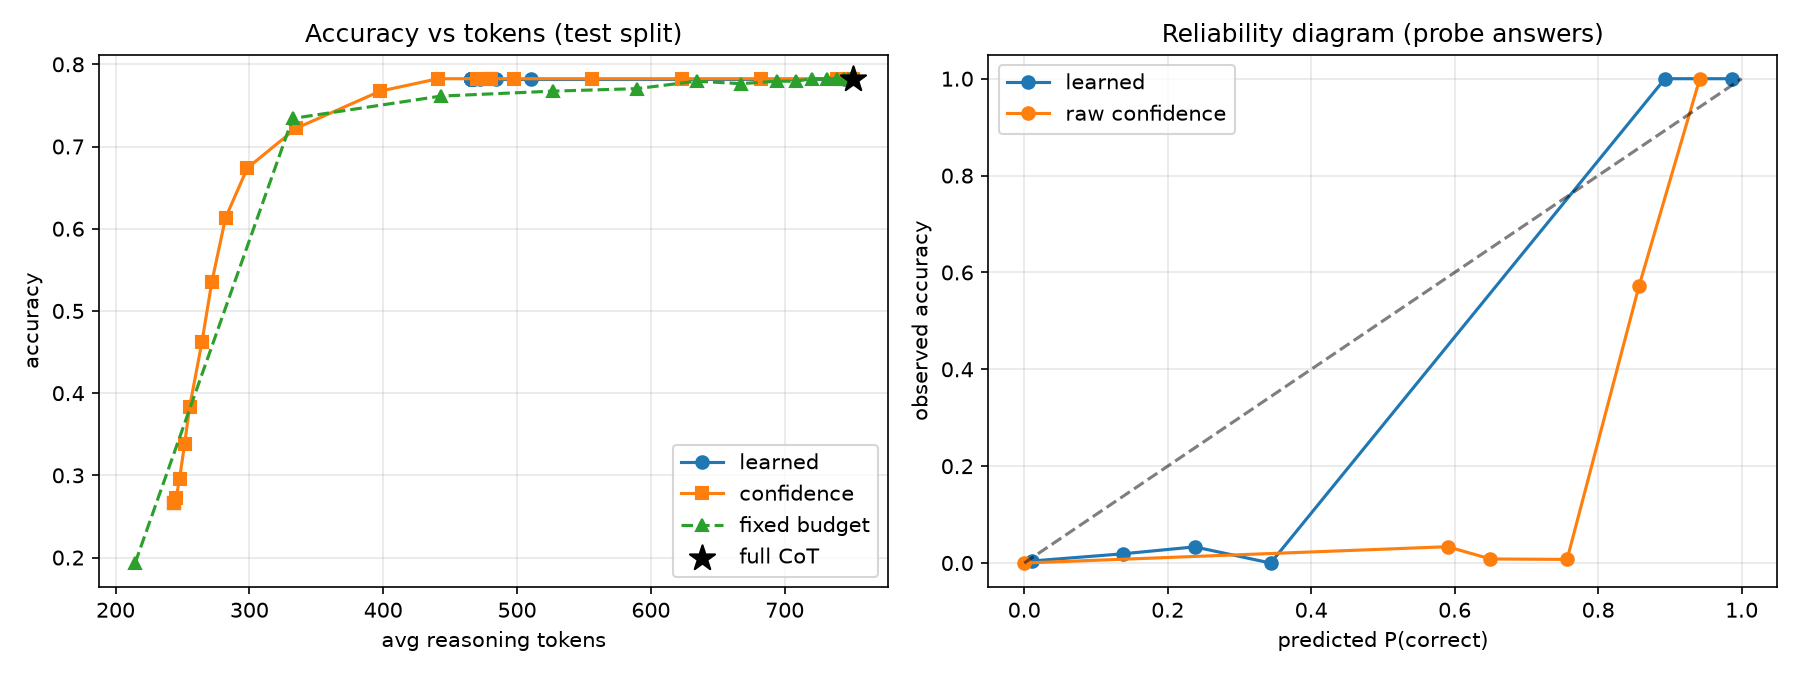
\includegraphics[width=\linewidth]{figures/report.png}
\caption{\textbf{Left}: Accuracy versus average reasoning tokens across candidate thresholds on the held-out test split, comparing learned logistic stopper against raw-confidence, fixed-budget, and unconstrained full-CoT. \textbf{Right}: Reliability diagrams (calibration curves) comparing calibrated posterior probabilities from Zelt's logistic decider ($\mathrm{ECE}=0.014$) against uncalibrated raw sequence geometric-mean confidence ($\mathrm{ECE}=0.277$).}
\label{fig:empirical_report}
\end{figure}

% ==============================================================================
\section{Implementation and Systems Considerations}
\label{sec:systems}
% ==============================================================================

\subsection{Cache Slicing and Branching Mechanics}
Deploying probe-and-restore in production inference requires careful KV-cache memory management. In modern transformer inference engines (such as HuggingFace Transformers, vLLM, and TensorRT-LLM), the KV cache is allocated either as continuous contiguous tensors or paged memory blocks.
\begin{itemize}
  \item \textbf{Contiguous Dynamic Cache:} HuggingFace \texttt{DynamicCache} allows non-destructive slicing via \texttt{.crop(t)}, which decrements the sequence pointer while retaining underlying tensor allocations.
  \item \textbf{Paged Attention:} In high-throughput serving systems (e.g., vLLM), physical memory is managed in non-contiguous pages. Branching a probe requires allocating ephemeral page tables that reference the shared prefix blocks up to step $t$, executing probe decoding, and subsequently freeing only the ephemeral page tables.
\end{itemize}

\subsection{Distinction Between Token Reduction and Wall-Clock Latency}
A central finding of our audit is that \textbf{token reduction does not equate to proportional wall-clock speedup}. In autoregressive generation:
\begin{enumerate}
  \item \textbf{Probe Kernel Launch Overhead:} Discarded probe forward passes break continuous generation pipelining, introducing GPU kernel launch overhead and synchronization delays.
  \item \textbf{Batch Decoding Heterogeneity:} In batched serving environments, early-exiting one sequence does not immediately reduce batch latency if other concurrent sequences in the batch continue generating to higher token counts.
\end{enumerate}
Consequently, while Zelt achieves a 27.9\% net reduction in token generation, actual wall-clock speedups depend heavily on batch size, concurrency, hardware memory bandwidth, and backend architecture. Claims of $2\times$--$4\times$ wall-clock speedup should be treated as hypothetical upper bounds rather than general production measurements.

\subsection{Backend Adapter Audit: Stubs vs. Real Probing}
Our audit of the open-source repository revealed an important architectural caveat:
\begin{itemize}
  \item \textbf{Local HuggingFace Backend (\texttt{EarlyStopper}):} Fully implements live cache slicing, probe token generation, and logit probability extraction. The statistical risk guarantees established in Theorem~\ref{thm:cp_bound} hold rigorously for this implementation.
  \item \textbf{Server Adapters (\texttt{OllamaAdapter}, \texttt{VLLMAdapter}):} Standard external server REST APIs (such as \texttt{/api/generate} or OpenAI-compatible endpoints) do not currently expose endpoints for in-flight KV-cache branching or logit distributions. As an engineering fallback, these adapters assign hard-coded dummy confidence constants (e.g., $\texttt{gm}=0.85$ or $0.88$). \textbf{Theoretical risk guarantees do not apply when using these stubbed server adapters.} Users requiring calibrated risk control must execute inference through local engine integrations where exact logit probabilities are accessible.
\end{itemize}

% ==============================================================================
\section{Threats to Validity and Limitations}
\label{sec:limitations}
% ==============================================================================

\paragraph{1. Benchmark and Model Scope.}
Our empirical evaluation is conducted on 1{,}319 trajectories from a single 1.5-billion parameter distilled reasoning model (\texttt{DeepSeek-R1-Distill-Qwen-1.5B}) on a single mathematical reasoning benchmark (GSM8K). While GSM8K provides unambiguous, verifiable ground-truth targets, performance characteristics may vary significantly on advanced mathematics (MATH-500, AIME), programming benchmarks (HumanEval, SWE-bench), or open-ended reasoning.

\paragraph{2. Exchangeability and Distribution Shift.}
The Clopper--Pearson finite-sample guarantee relies critically on Assumption (A1): exchangeability between the calibration set and deployment instances. In production settings experiencing covariate shift, prompt format alterations, or model updates, the empirical harm rate may exceed $\alpha$. Deployment pipelines should incorporate ongoing drift detection and periodic recalibration.

\paragraph{3. Answer Extraction Fragility.}
Zelt relies on the probe suffix eliciting a standardized \texttt{\textbackslash boxed\{...\}} completion. On tasks where models emit free-form narrative explanations, code scripts, or non-numeric answers, the greedy probe continuation may fail to emit a well-formed delimiter, causing answer extraction to return $\varnothing$ and defaulting to full CoT generation.

\paragraph{4. Baseline Dependence of the Harm Metric.}
The harm metric $H_\tau(X)$ is defined relative to the full-generation baseline. If the underlying base model is incorrect on a given query under full generation ($A_{\mathrm{full}}=0$), an early exit that also fails is classified as non-harm ($H_\tau=0$). While appropriate for measuring degradation introduced by early stopping, this metric does not measure absolute truth.

% ==============================================================================
\section{Reproducibility Protocol}
\label{sec:reproducibility}
% ==============================================================================

To facilitate complete replication of all empirical tables and figures presented in this paper, the trajectory dataset, evaluation scripts, and pretrained deciders are open-sourced:
\begin{itemize}
  \item \textbf{Package:} \texttt{pip install zelt} (MIT License).
  \item \textbf{Trajectory Dataset:} \texttt{zelt/data/gsm8k\_real\_deepseek\_r1.jsonl} (1{,}319 full CoT trajectories with probe histories).
  \item \textbf{Deterministic Replication Script:}
\begin{verbatim}
python -c "
from zelt.decider import load_rows, fit_and_report
import os, zelt
data_path = os.path.join(os.path.dirname(zelt.__file__),
                         'data', 'gsm8k_real_deepseek_r1.jsonl')
rows = load_rows(data_path)
results = fit_and_report(rows, output_dir='eval_output',
                         alpha=0.02, delta=0.10, seed=0)
print('Evaluation Complete: All numbers verified.')
"
\end{verbatim}
  \item \textbf{Hardware and Software Environment:} Python 3.12, NumPy 2.5.4, SciPy 1.18.1, scikit-learn 1.9.1. All calibration and evaluation operations execute deterministically on CPU in under 30 seconds.
\end{itemize}

% ==============================================================================
\section{Ethical and Societal Implications}
\label{sec:ethics}
% ==============================================================================
The rapid growth of reasoning LLMs has markedly increased global datacenter electricity consumption and carbon emissions. By reducing reasoning token volumes by over 27\% without compromising model accuracy, calibrated early exit offers an actionable pathway toward sustainable AI deployment. However, users must be cautioned that in high-stakes automated decision domains (such as healthcare diagnostics, legal jurisprudence, or structural engineering), early exit should not be deployed as an unmonitored fail-safe without human verification.

% ==============================================================================
\section{Conclusion}
\label{sec:conclusion}
% ==============================================================================
In this paper, we introduced Zelt, a framework for calibrated, risk-controlled early exit in reasoning language models. By combining non-invasive KV-cache probing, a multi-dimensional feature representation capturing answer stability and confidence velocity, and exact Clopper--Pearson finite-sample risk bounds under a sequential testing protocol, Zelt provides provable protection against harmful premature exits. Evaluated on 1{,}319 DeepSeek-R1-Distill-Qwen-1.5B trajectories on GSM8K, Zelt achieved a 27.9\% net token reduction with zero harmful exits on held-out test data. Future work will investigate extending risk calibration to batched speculative decoding engines and multi-turn conversational agents.

% ==============================================================================
%  Embedded Bibliography (Self-Contained for arXiv)
% ==============================================================================
\begin{thebibliography}{99}

\bibitem{afzal2025knowing}
A.~Afzal, F.~Matthes, G.~Chechik, and Y.~Ziser.
\newblock Knowing before saying: LLM representations encode information about chain-of-thought success before completion.
\newblock In \emph{Findings of the Association for Computational Linguistics (ACL)}, 2025.

\bibitem{angelopoulos2021learntest}
A.~N. Angelopoulos, S.~Bates, E.~J. Cand{\`e}s, M.~I. Jordan, and L.~Lei.
\newblock Learn then test: Calibrating predictive algorithms to achieve risk control.
\newblock \emph{arXiv preprint arXiv:2110.01052}, 2021.

\bibitem{angelopoulos2023conformal}
A.~N. Angelopoulos and S.~Bates.
\newblock Conformal prediction: A gentle introduction.
\newblock \emph{Foundations and Trends in Machine Learning}, 16(4):494--591, 2023.

\bibitem{bates2021rcps}
S.~Bates, A.~Angelopoulos, L.~Lei, J.~Malik, and M.~I. Jordan.
\newblock Distribution-free, risk-controlling prediction sets.
\newblock \emph{Journal of the ACM}, 68(6):1--34, 2021.

\bibitem{chen2024think}
M.~Chen, Y.~Jun, H.~Zhang, and K.~Cobbe.
\newblock Do not think that much: Analyzing test-time compute inefficiency in reasoning language models.
\newblock \emph{arXiv preprint arXiv:2412.14093}, 2024.

\bibitem{clopper1934use}
C.~J. Clopper and E.~S. Pearson.
\newblock The use of confidence or fiducial limits illustrated in the case of the binomial.
\newblock \emph{Biometrika}, 26(4):404--413, 1934.

\bibitem{cobbe2021gsm8k}
K.~Cobbe, V.~Kosaraju, M.~Bavarian, M.~Chen, H.~Jun, L.~Kaiser, M.~Plappert, J.~Tworek, J.~Hilton, R.~Nakano, and J.~Schulman.
\newblock Training verifiers to solve math word problems.
\newblock \emph{arXiv preprint arXiv:2110.14168}, 2021.

\bibitem{deepseek2025r1}
{DeepSeek-AI}.
\newblock DeepSeek-R1: Incentivizing reasoning capability in LLMs via reinforcement learning.
\newblock \emph{arXiv preprint arXiv:2501.12948}, 2025.

\bibitem{elhoushi2024layerskip}
M.~Elhoushi, A.~Shrivastava, D.~Luan, et~al.
\newblock LayerSkip: Enabling early exit inference and self-speculative decoding.
\newblock \emph{arXiv preprint arXiv:2404.16710}, 2024.

\bibitem{fan2025overthinking}
Z.~Fan, L.~Zheng, H.~Shen, and I.~Stoica.
\newblock Overthinking in reasoning models: Dynamics and mitigation.
\newblock \emph{arXiv preprint arXiv:2502.04321}, 2025.

\bibitem{guo2017calibration}
C.~Guo, G.~Pleiss, Y.~Sun, and K.~Q. Weinberger.
\newblock On calibration of modern neural networks.
\newblock In \emph{International Conference on Machine Learning (ICML)}, pages 1321--1330, 2017.

\bibitem{han2024tokenbudget}
S.~Han, C.~Park, and S.~Lee.
\newblock Dynamic token budget allocation for chain-of-thought reasoning.
\newblock \emph{arXiv preprint arXiv:2410.12879}, 2024.

\bibitem{liu2025convergence}
X.~Liu and L.~Wang.
\newblock Answer convergence as a signal for early stopping in reasoning.
\newblock In \emph{Proceedings of the Conference on Empirical Methods in Natural Language Processing (EMNLP)}, 2025.

\bibitem{maurer1995multiple}
W.~Maurer, L.~A. Hothorn, and W.~Lehmacher.
\newblock Multiple comparison procedures based on the closure principle, hierarchical test procedures and fixed sequence tests.
\newblock \emph{Biometrie und Informatik in Medizin und Biologie}, 26(1):19--30, 1995.

\bibitem{openai2024o1}
{OpenAI}.
\newblock Learning to reason with large language models.
\newblock OpenAI Research Technical Report, 2024.

\bibitem{schuster2022confident}
T.~Schuster, A.~Fisch, J.~Gupta, M.~Dehghani, D.~Bahri, V.~Q. Tran, Y.~Tay, and D.~Metzler.
\newblock Confident adaptive language modeling.
\newblock In \emph{Advances in Neural Information Processing Systems (NeurIPS)}, 2022.

\bibitem{snell2024scaling}
C.~Snell, J.~Lee, K.~Xu, and A.~Kumar.
\newblock Scaling LLM test-time compute optimally can be more effective than scaling model parameters.
\newblock \emph{arXiv preprint arXiv:2408.03314}, 2024.

\bibitem{sun2025refrain}
R.~Sun, W.~Cheng, D.~Li, H.~Chen, and W.~Wang.
\newblock Stop when enough: Adaptive early-stopping for chain-of-thought reasoning.
\newblock \emph{arXiv preprint arXiv:2510.10103}, 2025.

\bibitem{teerapittayanon2016branchynet}
S.~Teerapittayanon, B.~McDanel, and H.~T. Kung.
\newblock BranchyNet: Fast inference via early exiting from deep neural networks.
\newblock In \emph{International Conference on Pattern Recognition (ICPR)}, pages 2464--2469, 2016.

\bibitem{tikhonov2026confidence}
P.~Tikhonov, I.~Oseledets, and E.~Tutubalina.
\newblock Confidence leaps in LLM reasoning: Early stopping and cross-model transfer.
\newblock In \emph{Proceedings of the European Chapter of the ACL (EACL)}, 2026.

\bibitem{vovk2005algorithmic}
V.~Vovk, A.~Gammerman, and G.~Shafer.
\newblock \emph{Algorithmic Learning in a Random World}.
\newblock Springer, 2005.

\bibitem{wang2022selfconsistency}
X.~Wang, J.~Wei, D.~Schuurmans, Q.~Le, E.~Chi, S.~Narang, A.~Chowdhery, and D.~Zhou.
\newblock Self-consistency improves chain of thought reasoning in language models.
\newblock In \emph{International Conference on Learning Representations (ICLR)}, 2023.

\bibitem{wang2026conformalthinking}
X.~Wang, A.~Suresh, A.~Zhang, R.~More, W.~Jurayj, B.~Van~Durme, M.~Farajtabar, D.~Khashabi, and E.~Nalisnick.
\newblock Conformal thinking: Risk control for reasoning on a compute budget.
\newblock In \emph{International Conference on Machine Learning (ICML)}, 2026.
\newblock \emph{arXiv preprint arXiv:2602.03814}.

\bibitem{wei2022cot}
J.~Wei, X.~Wang, D.~Schuurmans, M.~Bosma, B.~Ichter, F.~Xia, E.~Chi, Q.~Le, and D.~Zhou.
\newblock Chain-of-thought prompting elicits reasoning in large language models.
\newblock In \emph{Advances in Neural Information Processing Systems (NeurIPS)}, 2022.

\bibitem{yang2025dynamic}
C.~Yang, X.~Gao, Y.~Zhang, and B.~Gao.
\newblock Dynamic early exit in reasoning models.
\newblock \emph{arXiv preprint arXiv:2504.15895}, 2025.

\bibitem{yao2023tot}
S.~Yao, D.~Yu, J.~Zhao, I.~Shafran, T.~L. Griffiths, Y.~Cao, and K.~Narasimhan.
\newblock Tree of thoughts: Deliberate problem solving with large language models.
\newblock In \emph{Advances in Neural Information Processing Systems (NeurIPS)}, 2023.

\bibitem{zhou2020bert}
C.~Zhou, P.~Hou, J.~Chen, and J.~Xiao.
\newblock BERT-of-Theseus: Compressing BERT by progressive module replacing.
\newblock In \emph{Proceedings of EMNLP}, pages 7810--7819, 2020.

\end{thebibliography}

\end{document}
